% Created by tikzDevice version 0.6.2-92-0ad2792 on 2013-11-12 07:31:04
% !TEX encoding = UTF-8 Unicode
\documentclass[12pt, mainfont = Minion,     mainscale = 1.0, sansfont = Myriad,     sansscale = MatchLowercase, monofont = Consolas,   monoscale = MatchLowercase, mathfont = MinionMath, mathscale = 1.0]{mtikzfig}
\begin{document}

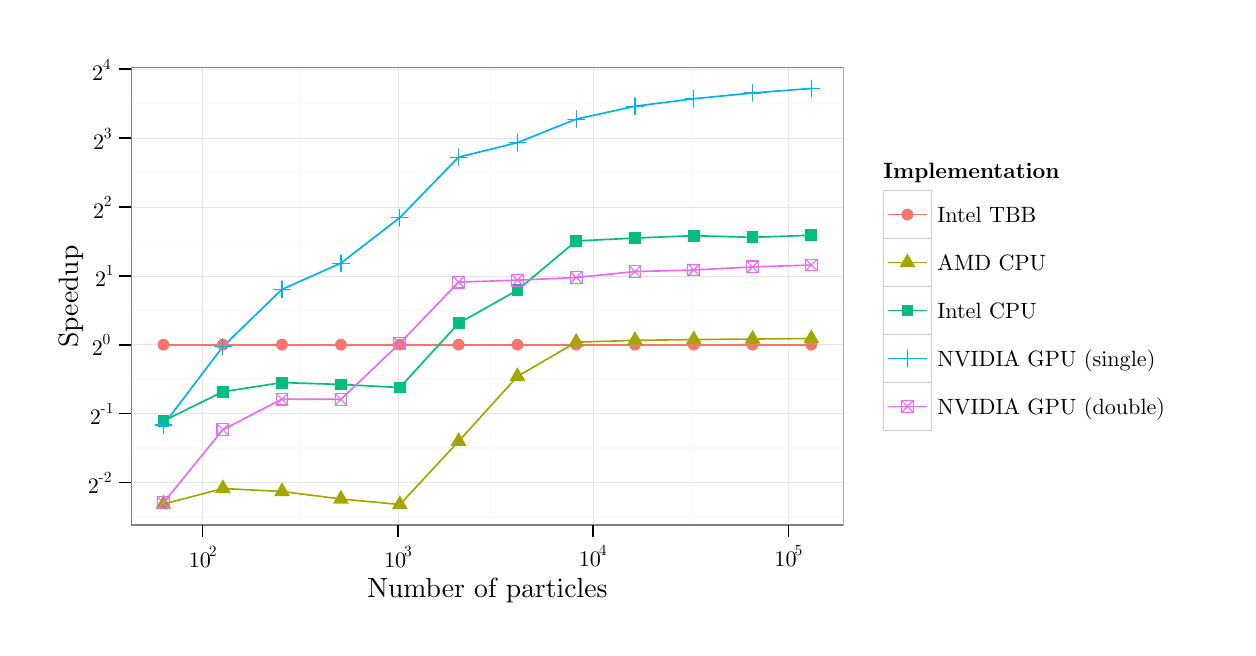
\begin{tikzpicture}[x=1pt,y=1pt]
\definecolor[named]{fillColor}{rgb}{1.00,1.00,1.00}
\path[use as bounding box,fill=fillColor,fill opacity=0.00] (0,0) rectangle (433.62,216.81);
\begin{scope}
\path[clip] (  0.00,  0.00) rectangle (433.62,216.81);
\definecolor[named]{drawColor}{rgb}{1.00,1.00,1.00}
\definecolor[named]{fillColor}{rgb}{1.00,1.00,1.00}

\path[draw=drawColor,line width= 0.6pt,line join=round,line cap=round,fill=fillColor] (  0.00,  0.00) rectangle (433.62,216.81);
\end{scope}
\begin{scope}
\path[clip] ( 37.35, 37.00) rectangle (294.88,202.36);
\definecolor[named]{fillColor}{rgb}{1.00,1.00,1.00}

\path[fill=fillColor] ( 37.35, 37.00) rectangle (294.88,202.36);
\definecolor[named]{drawColor}{rgb}{0.98,0.98,0.98}

\path[draw=drawColor,line width= 0.6pt,line join=round] ( 37.35, 40.05) --
	(294.88, 40.05);

\path[draw=drawColor,line width= 0.6pt,line join=round] ( 37.35, 64.93) --
	(294.88, 64.93);

\path[draw=drawColor,line width= 0.6pt,line join=round] ( 37.35, 89.82) --
	(294.88, 89.82);

\path[draw=drawColor,line width= 0.6pt,line join=round] ( 37.35,114.71) --
	(294.88,114.71);

\path[draw=drawColor,line width= 0.6pt,line join=round] ( 37.35,139.60) --
	(294.88,139.60);

\path[draw=drawColor,line width= 0.6pt,line join=round] ( 37.35,164.48) --
	(294.88,164.48);

\path[draw=drawColor,line width= 0.6pt,line join=round] ( 37.35,189.37) --
	(294.88,189.37);

\path[draw=drawColor,line width= 0.6pt,line join=round] ( 98.50, 37.00) --
	( 98.50,202.36);

\path[draw=drawColor,line width= 0.6pt,line join=round] (169.05, 37.00) --
	(169.05,202.36);

\path[draw=drawColor,line width= 0.6pt,line join=round] (239.60, 37.00) --
	(239.60,202.36);
\definecolor[named]{drawColor}{rgb}{0.90,0.90,0.90}

\path[draw=drawColor,line width= 0.2pt,line join=round] ( 37.35, 52.49) --
	(294.88, 52.49);

\path[draw=drawColor,line width= 0.2pt,line join=round] ( 37.35, 77.38) --
	(294.88, 77.38);

\path[draw=drawColor,line width= 0.2pt,line join=round] ( 37.35,102.26) --
	(294.88,102.26);

\path[draw=drawColor,line width= 0.2pt,line join=round] ( 37.35,127.15) --
	(294.88,127.15);

\path[draw=drawColor,line width= 0.2pt,line join=round] ( 37.35,152.04) --
	(294.88,152.04);

\path[draw=drawColor,line width= 0.2pt,line join=round] ( 37.35,176.93) --
	(294.88,176.93);

\path[draw=drawColor,line width= 0.2pt,line join=round] ( 37.35,201.81) --
	(294.88,201.81);

\path[draw=drawColor,line width= 0.2pt,line join=round] ( 63.22, 37.00) --
	( 63.22,202.36);

\path[draw=drawColor,line width= 0.2pt,line join=round] (133.77, 37.00) --
	(133.77,202.36);

\path[draw=drawColor,line width= 0.2pt,line join=round] (204.33, 37.00) --
	(204.33,202.36);

\path[draw=drawColor,line width= 0.2pt,line join=round] (274.88, 37.00) --
	(274.88,202.36);
\definecolor[named]{drawColor}{rgb}{0.97,0.46,0.43}

\path[draw=drawColor,line width= 0.6pt,line join=round] ( 49.06,102.26) --
	( 70.54,102.26) --
	( 91.90,102.26) --
	(113.20,102.26) --
	(134.47,102.26) --
	(155.72,102.26) --
	(176.97,102.26) --
	(198.21,102.26) --
	(219.45,102.26) --
	(240.69,102.26) --
	(261.93,102.26) --
	(283.17,102.26);
\definecolor[named]{drawColor}{rgb}{0.64,0.65,0.00}

\path[draw=drawColor,line width= 0.6pt,line join=round] ( 49.06, 44.64) --
	( 70.54, 50.29) --
	( 91.90, 49.20) --
	(113.20, 46.51) --
	(134.47, 44.51) --
	(155.72, 67.33) --
	(176.97, 90.79) --
	(198.21,103.17) --
	(219.45,103.82) --
	(240.69,104.10) --
	(261.93,104.30) --
	(283.17,104.49);
\definecolor[named]{drawColor}{rgb}{0.00,0.75,0.49}

\path[draw=drawColor,line width= 0.6pt,line join=round] ( 49.06, 74.69) --
	( 70.54, 85.25) --
	( 91.90, 88.56) --
	(113.20, 87.89) --
	(134.47, 86.78) --
	(155.72,109.99) --
	(176.97,121.94) --
	(198.21,139.74) --
	(219.45,140.78) --
	(240.69,141.65) --
	(261.93,141.05) --
	(283.17,141.80);
\definecolor[named]{drawColor}{rgb}{0.00,0.69,0.96}

\path[draw=drawColor,line width= 0.6pt,line join=round] ( 49.06, 73.24) --
	( 70.54,101.55) --
	( 91.90,122.26) --
	(113.20,131.71) --
	(134.47,148.16) --
	(155.72,170.02) --
	(176.97,175.26) --
	(198.21,183.76) --
	(219.45,188.42) --
	(240.69,191.12) --
	(261.93,193.21) --
	(283.17,194.84);
\definecolor[named]{drawColor}{rgb}{0.91,0.42,0.95}

\path[draw=drawColor,line width= 0.6pt,line join=round] ( 49.06, 45.12) --
	( 70.54, 71.53) --
	( 91.90, 82.59) --
	(113.20, 82.50) --
	(134.47,102.74) --
	(155.72,124.87) --
	(176.97,125.57) --
	(198.21,126.54) --
	(219.45,128.67) --
	(240.69,129.24) --
	(261.93,130.36) --
	(283.17,131.04);
\definecolor[named]{fillColor}{rgb}{0.97,0.46,0.43}

\path[fill=fillColor] ( 49.06,102.26) circle (  2.13);
\definecolor[named]{fillColor}{rgb}{0.64,0.65,0.00}

\path[fill=fillColor] ( 49.06, 47.96) --
	( 51.93, 42.98) --
	( 46.19, 42.98) --
	cycle;
\definecolor[named]{fillColor}{rgb}{0.00,0.75,0.49}

\path[fill=fillColor] ( 46.93, 72.55) --
	( 51.19, 72.55) --
	( 51.19, 76.82) --
	( 46.93, 76.82) --
	cycle;
\definecolor[named]{drawColor}{rgb}{0.00,0.69,0.96}

\path[draw=drawColor,line width= 0.4pt,line join=round,line cap=round] ( 46.04, 73.24) -- ( 52.08, 73.24);

\path[draw=drawColor,line width= 0.4pt,line join=round,line cap=round] ( 49.06, 70.22) -- ( 49.06, 76.25);
\definecolor[named]{drawColor}{rgb}{0.91,0.42,0.95}

\path[draw=drawColor,line width= 0.4pt,line join=round,line cap=round] ( 46.93, 42.99) rectangle ( 51.19, 47.26);

\path[draw=drawColor,line width= 0.4pt,line join=round,line cap=round] ( 46.93, 42.99) -- ( 51.19, 47.26);

\path[draw=drawColor,line width= 0.4pt,line join=round,line cap=round] ( 46.93, 47.26) -- ( 51.19, 42.99);
\definecolor[named]{fillColor}{rgb}{0.97,0.46,0.43}

\path[fill=fillColor] ( 70.54,102.26) circle (  2.13);
\definecolor[named]{fillColor}{rgb}{0.64,0.65,0.00}

\path[fill=fillColor] ( 70.54, 53.61) --
	( 73.42, 48.63) --
	( 67.67, 48.63) --
	cycle;
\definecolor[named]{fillColor}{rgb}{0.00,0.75,0.49}

\path[fill=fillColor] ( 68.41, 83.12) --
	( 72.68, 83.12) --
	( 72.68, 87.39) --
	( 68.41, 87.39) --
	cycle;
\definecolor[named]{drawColor}{rgb}{0.00,0.69,0.96}

\path[draw=drawColor,line width= 0.4pt,line join=round,line cap=round] ( 67.52,101.55) -- ( 73.56,101.55);

\path[draw=drawColor,line width= 0.4pt,line join=round,line cap=round] ( 70.54, 98.53) -- ( 70.54,104.56);
\definecolor[named]{drawColor}{rgb}{0.91,0.42,0.95}

\path[draw=drawColor,line width= 0.4pt,line join=round,line cap=round] ( 68.41, 69.40) rectangle ( 72.68, 73.67);

\path[draw=drawColor,line width= 0.4pt,line join=round,line cap=round] ( 68.41, 69.40) -- ( 72.68, 73.67);

\path[draw=drawColor,line width= 0.4pt,line join=round,line cap=round] ( 68.41, 73.67) -- ( 72.68, 69.40);
\definecolor[named]{fillColor}{rgb}{0.97,0.46,0.43}

\path[fill=fillColor] ( 91.90,102.26) circle (  2.13);
\definecolor[named]{fillColor}{rgb}{0.64,0.65,0.00}

\path[fill=fillColor] ( 91.90, 52.52) --
	( 94.78, 47.54) --
	( 89.03, 47.54) --
	cycle;
\definecolor[named]{fillColor}{rgb}{0.00,0.75,0.49}

\path[fill=fillColor] ( 89.77, 86.42) --
	( 94.04, 86.42) --
	( 94.04, 90.69) --
	( 89.77, 90.69) --
	cycle;
\definecolor[named]{drawColor}{rgb}{0.00,0.69,0.96}

\path[draw=drawColor,line width= 0.4pt,line join=round,line cap=round] ( 88.88,122.26) -- ( 94.92,122.26);

\path[draw=drawColor,line width= 0.4pt,line join=round,line cap=round] ( 91.90,119.24) -- ( 91.90,125.28);
\definecolor[named]{drawColor}{rgb}{0.91,0.42,0.95}

\path[draw=drawColor,line width= 0.4pt,line join=round,line cap=round] ( 89.77, 80.46) rectangle ( 94.04, 84.72);

\path[draw=drawColor,line width= 0.4pt,line join=round,line cap=round] ( 89.77, 80.46) -- ( 94.04, 84.72);

\path[draw=drawColor,line width= 0.4pt,line join=round,line cap=round] ( 89.77, 84.72) -- ( 94.04, 80.46);
\definecolor[named]{fillColor}{rgb}{0.97,0.46,0.43}

\path[fill=fillColor] (113.20,102.26) circle (  2.13);
\definecolor[named]{fillColor}{rgb}{0.64,0.65,0.00}

\path[fill=fillColor] (113.20, 49.83) --
	(116.07, 44.85) --
	(110.33, 44.85) --
	cycle;
\definecolor[named]{fillColor}{rgb}{0.00,0.75,0.49}

\path[fill=fillColor] (111.07, 85.76) --
	(115.33, 85.76) --
	(115.33, 90.02) --
	(111.07, 90.02) --
	cycle;
\definecolor[named]{drawColor}{rgb}{0.00,0.69,0.96}

\path[draw=drawColor,line width= 0.4pt,line join=round,line cap=round] (110.18,131.71) -- (116.22,131.71);

\path[draw=drawColor,line width= 0.4pt,line join=round,line cap=round] (113.20,128.69) -- (113.20,134.73);
\definecolor[named]{drawColor}{rgb}{0.91,0.42,0.95}

\path[draw=drawColor,line width= 0.4pt,line join=round,line cap=round] (111.07, 80.37) rectangle (115.33, 84.64);

\path[draw=drawColor,line width= 0.4pt,line join=round,line cap=round] (111.07, 80.37) -- (115.33, 84.64);

\path[draw=drawColor,line width= 0.4pt,line join=round,line cap=round] (111.07, 84.64) -- (115.33, 80.37);
\definecolor[named]{fillColor}{rgb}{0.97,0.46,0.43}

\path[fill=fillColor] (134.47,102.26) circle (  2.13);
\definecolor[named]{fillColor}{rgb}{0.64,0.65,0.00}

\path[fill=fillColor] (134.47, 47.83) --
	(137.34, 42.85) --
	(131.60, 42.85) --
	cycle;
\definecolor[named]{fillColor}{rgb}{0.00,0.75,0.49}

\path[fill=fillColor] (132.34, 84.65) --
	(136.60, 84.65) --
	(136.60, 88.92) --
	(132.34, 88.92) --
	cycle;
\definecolor[named]{drawColor}{rgb}{0.00,0.69,0.96}

\path[draw=drawColor,line width= 0.4pt,line join=round,line cap=round] (131.45,148.16) -- (137.49,148.16);

\path[draw=drawColor,line width= 0.4pt,line join=round,line cap=round] (134.47,145.15) -- (134.47,151.18);
\definecolor[named]{drawColor}{rgb}{0.91,0.42,0.95}

\path[draw=drawColor,line width= 0.4pt,line join=round,line cap=round] (132.34,100.60) rectangle (136.60,104.87);

\path[draw=drawColor,line width= 0.4pt,line join=round,line cap=round] (132.34,100.60) -- (136.60,104.87);

\path[draw=drawColor,line width= 0.4pt,line join=round,line cap=round] (132.34,104.87) -- (136.60,100.60);
\definecolor[named]{fillColor}{rgb}{0.97,0.46,0.43}

\path[fill=fillColor] (155.72,102.26) circle (  2.13);
\definecolor[named]{fillColor}{rgb}{0.64,0.65,0.00}

\path[fill=fillColor] (155.72, 70.65) --
	(158.60, 65.67) --
	(152.85, 65.67) --
	cycle;
\definecolor[named]{fillColor}{rgb}{0.00,0.75,0.49}

\path[fill=fillColor] (153.59,107.86) --
	(157.86,107.86) --
	(157.86,112.12) --
	(153.59,112.12) --
	cycle;
\definecolor[named]{drawColor}{rgb}{0.00,0.69,0.96}

\path[draw=drawColor,line width= 0.4pt,line join=round,line cap=round] (152.71,170.02) -- (158.74,170.02);

\path[draw=drawColor,line width= 0.4pt,line join=round,line cap=round] (155.72,167.00) -- (155.72,173.04);
\definecolor[named]{drawColor}{rgb}{0.91,0.42,0.95}

\path[draw=drawColor,line width= 0.4pt,line join=round,line cap=round] (153.59,122.73) rectangle (157.86,127.00);

\path[draw=drawColor,line width= 0.4pt,line join=round,line cap=round] (153.59,122.73) -- (157.86,127.00);

\path[draw=drawColor,line width= 0.4pt,line join=round,line cap=round] (153.59,127.00) -- (157.86,122.73);
\definecolor[named]{fillColor}{rgb}{0.97,0.46,0.43}

\path[fill=fillColor] (176.97,102.26) circle (  2.13);
\definecolor[named]{fillColor}{rgb}{0.64,0.65,0.00}

\path[fill=fillColor] (176.97, 94.11) --
	(179.84, 89.13) --
	(174.10, 89.13) --
	cycle;
\definecolor[named]{fillColor}{rgb}{0.00,0.75,0.49}

\path[fill=fillColor] (174.84,119.81) --
	(179.10,119.81) --
	(179.10,124.08) --
	(174.84,124.08) --
	cycle;
\definecolor[named]{drawColor}{rgb}{0.00,0.69,0.96}

\path[draw=drawColor,line width= 0.4pt,line join=round,line cap=round] (173.95,175.26) -- (179.99,175.26);

\path[draw=drawColor,line width= 0.4pt,line join=round,line cap=round] (176.97,172.24) -- (176.97,178.28);
\definecolor[named]{drawColor}{rgb}{0.91,0.42,0.95}

\path[draw=drawColor,line width= 0.4pt,line join=round,line cap=round] (174.84,123.44) rectangle (179.10,127.71);

\path[draw=drawColor,line width= 0.4pt,line join=round,line cap=round] (174.84,123.44) -- (179.10,127.71);

\path[draw=drawColor,line width= 0.4pt,line join=round,line cap=round] (174.84,127.71) -- (179.10,123.44);
\definecolor[named]{fillColor}{rgb}{0.97,0.46,0.43}

\path[fill=fillColor] (198.21,102.26) circle (  2.13);
\definecolor[named]{fillColor}{rgb}{0.64,0.65,0.00}

\path[fill=fillColor] (198.21,106.49) --
	(201.09,101.51) --
	(195.34,101.51) --
	cycle;
\definecolor[named]{fillColor}{rgb}{0.00,0.75,0.49}

\path[fill=fillColor] (196.08,137.61) --
	(200.35,137.61) --
	(200.35,141.87) --
	(196.08,141.87) --
	cycle;
\definecolor[named]{drawColor}{rgb}{0.00,0.69,0.96}

\path[draw=drawColor,line width= 0.4pt,line join=round,line cap=round] (195.19,183.76) -- (201.23,183.76);

\path[draw=drawColor,line width= 0.4pt,line join=round,line cap=round] (198.21,180.75) -- (198.21,186.78);
\definecolor[named]{drawColor}{rgb}{0.91,0.42,0.95}

\path[draw=drawColor,line width= 0.4pt,line join=round,line cap=round] (196.08,124.40) rectangle (200.35,128.67);

\path[draw=drawColor,line width= 0.4pt,line join=round,line cap=round] (196.08,124.40) -- (200.35,128.67);

\path[draw=drawColor,line width= 0.4pt,line join=round,line cap=round] (196.08,128.67) -- (200.35,124.40);
\definecolor[named]{fillColor}{rgb}{0.97,0.46,0.43}

\path[fill=fillColor] (219.45,102.26) circle (  2.13);
\definecolor[named]{fillColor}{rgb}{0.64,0.65,0.00}

\path[fill=fillColor] (219.45,107.14) --
	(222.33,102.16) --
	(216.58,102.16) --
	cycle;
\definecolor[named]{fillColor}{rgb}{0.00,0.75,0.49}

\path[fill=fillColor] (217.32,138.64) --
	(221.59,138.64) --
	(221.59,142.91) --
	(217.32,142.91) --
	cycle;
\definecolor[named]{drawColor}{rgb}{0.00,0.69,0.96}

\path[draw=drawColor,line width= 0.4pt,line join=round,line cap=round] (216.44,188.42) -- (222.47,188.42);

\path[draw=drawColor,line width= 0.4pt,line join=round,line cap=round] (219.45,185.41) -- (219.45,191.44);
\definecolor[named]{drawColor}{rgb}{0.91,0.42,0.95}

\path[draw=drawColor,line width= 0.4pt,line join=round,line cap=round] (217.32,126.54) rectangle (221.59,130.81);

\path[draw=drawColor,line width= 0.4pt,line join=round,line cap=round] (217.32,126.54) -- (221.59,130.81);

\path[draw=drawColor,line width= 0.4pt,line join=round,line cap=round] (217.32,130.81) -- (221.59,126.54);
\definecolor[named]{fillColor}{rgb}{0.97,0.46,0.43}

\path[fill=fillColor] (240.69,102.26) circle (  2.13);
\definecolor[named]{fillColor}{rgb}{0.64,0.65,0.00}

\path[fill=fillColor] (240.69,107.42) --
	(243.57,102.44) --
	(237.82,102.44) --
	cycle;
\definecolor[named]{fillColor}{rgb}{0.00,0.75,0.49}

\path[fill=fillColor] (238.56,139.52) --
	(242.83,139.52) --
	(242.83,143.79) --
	(238.56,143.79) --
	cycle;
\definecolor[named]{drawColor}{rgb}{0.00,0.69,0.96}

\path[draw=drawColor,line width= 0.4pt,line join=round,line cap=round] (237.68,191.12) -- (243.71,191.12);

\path[draw=drawColor,line width= 0.4pt,line join=round,line cap=round] (240.69,188.10) -- (240.69,194.13);
\definecolor[named]{drawColor}{rgb}{0.91,0.42,0.95}

\path[draw=drawColor,line width= 0.4pt,line join=round,line cap=round] (238.56,127.11) rectangle (242.83,131.38);

\path[draw=drawColor,line width= 0.4pt,line join=round,line cap=round] (238.56,127.11) -- (242.83,131.38);

\path[draw=drawColor,line width= 0.4pt,line join=round,line cap=round] (238.56,131.38) -- (242.83,127.11);
\definecolor[named]{fillColor}{rgb}{0.97,0.46,0.43}

\path[fill=fillColor] (261.93,102.26) circle (  2.13);
\definecolor[named]{fillColor}{rgb}{0.64,0.65,0.00}

\path[fill=fillColor] (261.93,107.62) --
	(264.81,102.64) --
	(259.06,102.64) --
	cycle;
\definecolor[named]{fillColor}{rgb}{0.00,0.75,0.49}

\path[fill=fillColor] (259.80,138.92) --
	(264.07,138.92) --
	(264.07,143.19) --
	(259.80,143.19) --
	cycle;
\definecolor[named]{drawColor}{rgb}{0.00,0.69,0.96}

\path[draw=drawColor,line width= 0.4pt,line join=round,line cap=round] (258.92,193.21) -- (264.95,193.21);

\path[draw=drawColor,line width= 0.4pt,line join=round,line cap=round] (261.93,190.19) -- (261.93,196.23);
\definecolor[named]{drawColor}{rgb}{0.91,0.42,0.95}

\path[draw=drawColor,line width= 0.4pt,line join=round,line cap=round] (259.80,128.22) rectangle (264.07,132.49);

\path[draw=drawColor,line width= 0.4pt,line join=round,line cap=round] (259.80,128.22) -- (264.07,132.49);

\path[draw=drawColor,line width= 0.4pt,line join=round,line cap=round] (259.80,132.49) -- (264.07,128.22);
\definecolor[named]{fillColor}{rgb}{0.97,0.46,0.43}

\path[fill=fillColor] (283.17,102.26) circle (  2.13);
\definecolor[named]{fillColor}{rgb}{0.64,0.65,0.00}

\path[fill=fillColor] (283.17,107.80) --
	(286.05,102.83) --
	(280.30,102.83) --
	cycle;
\definecolor[named]{fillColor}{rgb}{0.00,0.75,0.49}

\path[fill=fillColor] (281.04,139.66) --
	(285.31,139.66) --
	(285.31,143.93) --
	(281.04,143.93) --
	cycle;
\definecolor[named]{drawColor}{rgb}{0.00,0.69,0.96}

\path[draw=drawColor,line width= 0.4pt,line join=round,line cap=round] (280.15,194.84) -- (286.19,194.84);

\path[draw=drawColor,line width= 0.4pt,line join=round,line cap=round] (283.17,191.82) -- (283.17,197.86);
\definecolor[named]{drawColor}{rgb}{0.91,0.42,0.95}

\path[draw=drawColor,line width= 0.4pt,line join=round,line cap=round] (281.04,128.91) rectangle (285.31,133.17);

\path[draw=drawColor,line width= 0.4pt,line join=round,line cap=round] (281.04,128.91) -- (285.31,133.17);

\path[draw=drawColor,line width= 0.4pt,line join=round,line cap=round] (281.04,133.17) -- (285.31,128.91);
\definecolor[named]{drawColor}{rgb}{0.50,0.50,0.50}

\path[draw=drawColor,line width= 0.6pt,line join=round,line cap=round] ( 37.35, 37.00) rectangle (294.88,202.36);
\end{scope}
\begin{scope}
\path[clip] (  0.00,  0.00) rectangle (433.62,216.81);
\definecolor[named]{drawColor}{rgb}{0.00,0.00,0.00}

\node[text=drawColor,anchor=base west,inner sep=0pt, outer sep=0pt, scale=  0.80] at ( 21.77, 48.48) {2};

\node[text=drawColor,anchor=base west,inner sep=0pt, outer sep=0pt, scale=  0.56] at ( 25.66, 52.48) {-};

\node[text=drawColor,anchor=base west,inner sep=0pt, outer sep=0pt, scale=  0.56] at ( 27.52, 52.48) {2};

\node[text=drawColor,anchor=base west,inner sep=0pt, outer sep=0pt, scale=  0.80] at ( 22.51, 73.40) {2};

\node[text=drawColor,anchor=base west,inner sep=0pt, outer sep=0pt, scale=  0.56] at ( 26.39, 77.40) {-};

\node[text=drawColor,anchor=base west,inner sep=0pt, outer sep=0pt, scale=  0.56] at ( 28.26, 77.40) {1};

\node[text=drawColor,anchor=base west,inner sep=0pt, outer sep=0pt, scale=  0.80] at ( 23.24, 98.26) {2};

\node[text=drawColor,anchor=base west,inner sep=0pt, outer sep=0pt, scale=  0.56] at ( 27.12,102.25) {0};

\node[text=drawColor,anchor=base west,inner sep=0pt, outer sep=0pt, scale=  0.80] at ( 24.38,123.18) {2};

\node[text=drawColor,anchor=base west,inner sep=0pt, outer sep=0pt, scale=  0.56] at ( 28.26,127.17) {1};

\node[text=drawColor,anchor=base west,inner sep=0pt, outer sep=0pt, scale=  0.80] at ( 23.64,148.03) {2};

\node[text=drawColor,anchor=base west,inner sep=0pt, outer sep=0pt, scale=  0.56] at ( 27.52,152.03) {2};

\node[text=drawColor,anchor=base west,inner sep=0pt, outer sep=0pt, scale=  0.80] at ( 23.62,172.92) {2};

\node[text=drawColor,anchor=base west,inner sep=0pt, outer sep=0pt, scale=  0.56] at ( 27.51,176.91) {3};

\node[text=drawColor,anchor=base west,inner sep=0pt, outer sep=0pt, scale=  0.80] at ( 23.30,197.84) {2};

\node[text=drawColor,anchor=base west,inner sep=0pt, outer sep=0pt, scale=  0.56] at ( 27.18,201.84) {4};
\end{scope}
\begin{scope}
\path[clip] (  0.00,  0.00) rectangle (433.62,216.81);
\definecolor[named]{drawColor}{rgb}{0.00,0.00,0.00}

\path[draw=drawColor,line width= 0.6pt,line join=round] ( 33.09, 52.49) --
	( 37.35, 52.49);

\path[draw=drawColor,line width= 0.6pt,line join=round] ( 33.09, 77.38) --
	( 37.35, 77.38);

\path[draw=drawColor,line width= 0.6pt,line join=round] ( 33.09,102.26) --
	( 37.35,102.26);

\path[draw=drawColor,line width= 0.6pt,line join=round] ( 33.09,127.15) --
	( 37.35,127.15);

\path[draw=drawColor,line width= 0.6pt,line join=round] ( 33.09,152.04) --
	( 37.35,152.04);

\path[draw=drawColor,line width= 0.6pt,line join=round] ( 33.09,176.93) --
	( 37.35,176.93);

\path[draw=drawColor,line width= 0.6pt,line join=round] ( 33.09,201.81) --
	( 37.35,201.81);
\end{scope}
\begin{scope}
\path[clip] (  0.00,  0.00) rectangle (433.62,216.81);
\definecolor[named]{drawColor}{rgb}{0.00,0.00,0.00}

\path[draw=drawColor,line width= 0.6pt,line join=round] ( 63.22, 32.73) --
	( 63.22, 37.00);

\path[draw=drawColor,line width= 0.6pt,line join=round] (133.77, 32.73) --
	(133.77, 37.00);

\path[draw=drawColor,line width= 0.6pt,line join=round] (204.33, 32.73) --
	(204.33, 37.00);

\path[draw=drawColor,line width= 0.6pt,line join=round] (274.88, 32.73) --
	(274.88, 37.00);
\end{scope}
\begin{scope}
\path[clip] (  0.00,  0.00) rectangle (433.62,216.81);
\definecolor[named]{drawColor}{rgb}{0.00,0.00,0.00}

\node[text=drawColor,anchor=base west,inner sep=0pt, outer sep=0pt, scale=  0.80] at ( 58.21, 21.87) {10};

\node[text=drawColor,anchor=base west,inner sep=0pt, outer sep=0pt, scale=  0.56] at ( 65.50, 25.86) {2};

\node[text=drawColor,anchor=base west,inner sep=0pt, outer sep=0pt, scale=  0.80] at (128.76, 21.87) {10};

\node[text=drawColor,anchor=base west,inner sep=0pt, outer sep=0pt, scale=  0.56] at (136.05, 25.86) {3};

\node[text=drawColor,anchor=base west,inner sep=0pt, outer sep=0pt, scale=  0.80] at (199.15, 21.94) {10};

\node[text=drawColor,anchor=base west,inner sep=0pt, outer sep=0pt, scale=  0.56] at (206.44, 25.93) {4};

\node[text=drawColor,anchor=base west,inner sep=0pt, outer sep=0pt, scale=  0.80] at (269.84, 21.94) {10};

\node[text=drawColor,anchor=base west,inner sep=0pt, outer sep=0pt, scale=  0.56] at (277.13, 25.93) {5};
\end{scope}
\begin{scope}
\path[clip] (  0.00,  0.00) rectangle (433.62,216.81);
\definecolor[named]{drawColor}{rgb}{0.00,0.00,0.00}

\node[text=drawColor,anchor=base,inner sep=0pt, outer sep=0pt, scale=  1.00] at (166.12, 10.84) {Number of particles};
\end{scope}
\begin{scope}
\path[clip] (  0.00,  0.00) rectangle (433.62,216.81);
\definecolor[named]{drawColor}{rgb}{0.00,0.00,0.00}

\node[text=drawColor,rotate= 90.00,anchor=base,inner sep=0pt, outer sep=0pt, scale=  1.00] at ( 18.16,119.68) {Speedup};
\end{scope}
\begin{scope}
\path[clip] (  0.00,  0.00) rectangle (433.62,216.81);
\definecolor[named]{fillColor}{rgb}{1.00,1.00,1.00}

\path[fill=fillColor] (304.95, 66.95) rectangle (409.09,172.40);
\end{scope}
\begin{scope}
\path[clip] (  0.00,  0.00) rectangle (433.62,216.81);
\definecolor[named]{drawColor}{rgb}{0.00,0.00,0.00}

\node[text=drawColor,anchor=base west,inner sep=0pt, outer sep=0pt, scale=  0.80] at (309.22,162.28) {\bfseries Implementation};
\end{scope}
\begin{scope}
\path[clip] (  0.00,  0.00) rectangle (433.62,216.81);
\definecolor[named]{drawColor}{rgb}{0.80,0.80,0.80}
\definecolor[named]{fillColor}{rgb}{1.00,1.00,1.00}

\path[draw=drawColor,line width= 0.6pt,line join=round,line cap=round,fill=fillColor] (309.22,140.60) rectangle (326.56,157.94);
\end{scope}
\begin{scope}
\path[clip] (  0.00,  0.00) rectangle (433.62,216.81);
\definecolor[named]{drawColor}{rgb}{0.97,0.46,0.43}

\path[draw=drawColor,line width= 0.6pt,line join=round] (310.95,149.27) -- (324.83,149.27);
\end{scope}
\begin{scope}
\path[clip] (  0.00,  0.00) rectangle (433.62,216.81);
\definecolor[named]{fillColor}{rgb}{0.97,0.46,0.43}

\path[fill=fillColor] (317.89,149.27) circle (  2.13);
\end{scope}
\begin{scope}
\path[clip] (  0.00,  0.00) rectangle (433.62,216.81);
\definecolor[named]{drawColor}{rgb}{0.80,0.80,0.80}
\definecolor[named]{fillColor}{rgb}{1.00,1.00,1.00}

\path[draw=drawColor,line width= 0.6pt,line join=round,line cap=round,fill=fillColor] (309.22,123.25) rectangle (326.56,140.60);
\end{scope}
\begin{scope}
\path[clip] (  0.00,  0.00) rectangle (433.62,216.81);
\definecolor[named]{drawColor}{rgb}{0.64,0.65,0.00}

\path[draw=drawColor,line width= 0.6pt,line join=round] (310.95,131.93) -- (324.83,131.93);
\end{scope}
\begin{scope}
\path[clip] (  0.00,  0.00) rectangle (433.62,216.81);
\definecolor[named]{fillColor}{rgb}{0.64,0.65,0.00}

\path[fill=fillColor] (317.89,135.24) --
	(320.76,130.27) --
	(315.02,130.27) --
	cycle;
\end{scope}
\begin{scope}
\path[clip] (  0.00,  0.00) rectangle (433.62,216.81);
\definecolor[named]{drawColor}{rgb}{0.80,0.80,0.80}
\definecolor[named]{fillColor}{rgb}{1.00,1.00,1.00}

\path[draw=drawColor,line width= 0.6pt,line join=round,line cap=round,fill=fillColor] (309.22,105.91) rectangle (326.56,123.25);
\end{scope}
\begin{scope}
\path[clip] (  0.00,  0.00) rectangle (433.62,216.81);
\definecolor[named]{drawColor}{rgb}{0.00,0.75,0.49}

\path[draw=drawColor,line width= 0.6pt,line join=round] (310.95,114.58) -- (324.83,114.58);
\end{scope}
\begin{scope}
\path[clip] (  0.00,  0.00) rectangle (433.62,216.81);
\definecolor[named]{fillColor}{rgb}{0.00,0.75,0.49}

\path[fill=fillColor] (315.76,112.45) --
	(320.02,112.45) --
	(320.02,116.71) --
	(315.76,116.71) --
	cycle;
\end{scope}
\begin{scope}
\path[clip] (  0.00,  0.00) rectangle (433.62,216.81);
\definecolor[named]{drawColor}{rgb}{0.80,0.80,0.80}
\definecolor[named]{fillColor}{rgb}{1.00,1.00,1.00}

\path[draw=drawColor,line width= 0.6pt,line join=round,line cap=round,fill=fillColor] (309.22, 88.56) rectangle (326.56,105.91);
\end{scope}
\begin{scope}
\path[clip] (  0.00,  0.00) rectangle (433.62,216.81);
\definecolor[named]{drawColor}{rgb}{0.00,0.69,0.96}

\path[draw=drawColor,line width= 0.6pt,line join=round] (310.95, 97.24) -- (324.83, 97.24);
\end{scope}
\begin{scope}
\path[clip] (  0.00,  0.00) rectangle (433.62,216.81);
\definecolor[named]{drawColor}{rgb}{0.00,0.69,0.96}

\path[draw=drawColor,line width= 0.4pt,line join=round,line cap=round] (314.87, 97.24) -- (320.91, 97.24);

\path[draw=drawColor,line width= 0.4pt,line join=round,line cap=round] (317.89, 94.22) -- (317.89,100.25);
\end{scope}
\begin{scope}
\path[clip] (  0.00,  0.00) rectangle (433.62,216.81);
\definecolor[named]{drawColor}{rgb}{0.80,0.80,0.80}
\definecolor[named]{fillColor}{rgb}{1.00,1.00,1.00}

\path[draw=drawColor,line width= 0.6pt,line join=round,line cap=round,fill=fillColor] (309.22, 71.22) rectangle (326.56, 88.56);
\end{scope}
\begin{scope}
\path[clip] (  0.00,  0.00) rectangle (433.62,216.81);
\definecolor[named]{drawColor}{rgb}{0.91,0.42,0.95}

\path[draw=drawColor,line width= 0.6pt,line join=round] (310.95, 79.89) -- (324.83, 79.89);
\end{scope}
\begin{scope}
\path[clip] (  0.00,  0.00) rectangle (433.62,216.81);
\definecolor[named]{drawColor}{rgb}{0.91,0.42,0.95}

\path[draw=drawColor,line width= 0.4pt,line join=round,line cap=round] (315.76, 77.76) rectangle (320.02, 82.02);

\path[draw=drawColor,line width= 0.4pt,line join=round,line cap=round] (315.76, 77.76) -- (320.02, 82.02);

\path[draw=drawColor,line width= 0.4pt,line join=round,line cap=round] (315.76, 82.02) -- (320.02, 77.76);
\end{scope}
\begin{scope}
\path[clip] (  0.00,  0.00) rectangle (433.62,216.81);
\definecolor[named]{drawColor}{rgb}{0.00,0.00,0.00}

\node[text=drawColor,anchor=base west,inner sep=0pt, outer sep=0pt, scale=  0.80] at (328.73,146.34) {Intel TBB};
\end{scope}
\begin{scope}
\path[clip] (  0.00,  0.00) rectangle (433.62,216.81);
\definecolor[named]{drawColor}{rgb}{0.00,0.00,0.00}

\node[text=drawColor,anchor=base west,inner sep=0pt, outer sep=0pt, scale=  0.80] at (328.73,129.00) {AMD CPU};
\end{scope}
\begin{scope}
\path[clip] (  0.00,  0.00) rectangle (433.62,216.81);
\definecolor[named]{drawColor}{rgb}{0.00,0.00,0.00}

\node[text=drawColor,anchor=base west,inner sep=0pt, outer sep=0pt, scale=  0.80] at (328.73,111.65) {Intel CPU};
\end{scope}
\begin{scope}
\path[clip] (  0.00,  0.00) rectangle (433.62,216.81);
\definecolor[named]{drawColor}{rgb}{0.00,0.00,0.00}

\node[text=drawColor,anchor=base west,inner sep=0pt, outer sep=0pt, scale=  0.80] at (328.73, 94.31) {NVIDIA GPU (single)};
\end{scope}
\begin{scope}
\path[clip] (  0.00,  0.00) rectangle (433.62,216.81);
\definecolor[named]{drawColor}{rgb}{0.00,0.00,0.00}

\node[text=drawColor,anchor=base west,inner sep=0pt, outer sep=0pt, scale=  0.80] at (328.73, 76.96) {NVIDIA GPU (double)};
\end{scope}
\end{tikzpicture}

\end{document}
